\documentclass{beamer}
\usepackage{graphicx}
\usepackage{listings} % Syntax highlighing
\usepackage{fancyvrb} % Inline verbatim
\usepackage{hyperref} % Hyperlinks
\hypersetup{pdfpagemode=FullScreen}
\usepackage{tikz}

\usetheme{Boadilla}
\title{Logistic Regression}
\author{UMBC Malware Data Science}
\date{Week 11: 14 April 2020}

\begin{document}

\begin{frame}{Recap}
    Up until now, we've we've picked our features for the input vectors, be it domain-specific or $n$-grams. Let's instead use an algorithm to select the best features for us.
\end{frame}

\begin{frame}{Fitting}
    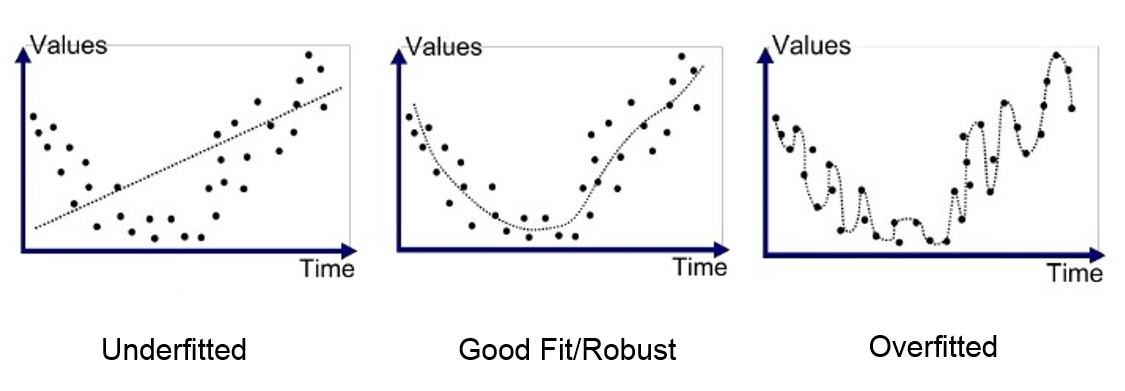
\includegraphics[scale=0.31]{Images/fitting.png}
    \\
    \footnotesize{Source: \url{https://medium.com/greyatom/what-is-underfitting-and-overfitting-in-machine-learning-and-how-to-deal-with-it-6803a989c76}}
\end{frame}

\begin{frame}{Logisitic Regression with Regularization}
    To counter overfitting, and noise which may be in the data, we can provide a penalty to the algorithm which helps build a better model.
    \begin{itemize}
        \item L1: Lasso pushes coefficients to exactly zero, potentially removing unneeded features
        \item L2: Ridge pushes coefficients to nearly zero, smoothing out the decision boundary
        \item L1+L2: Elastic Net, both Lasso and Ridge can be applied to get the best of both
    \end{itemize}
    These methods can be used to reduce the number of features in the dataset, making a smaller, easier to manage model. You may find that a model trained with Lasso and/or Ridge does worse on the training data, but better on the testing data.
\end{frame}

\begin{frame}{Real Use of ElasticNet}
    My team uses ElasticNet to train a malware detection model.
    \begin{itemize}
        \item We started by using a neural network and 2000 features.
        \item We tried a few different ways to pick the best features, with little impact on performance.
        \item We achieved much better success when we picked the top one million most common 6-grams, and later 8-grams, and let the algorithm decide on the best features.
        \item Our latest model has 96,000 features, down from one million, and they're likely much better than anything we or another human could have chosen.
    \end{itemize}
\end{frame}

\begin{frame}{Pandas}
    Pandas is a Python module which makes it easier to handle data. We'll use it to read in CSV files, and to train models. The dataframe is a giant matrix which makes it easy to add or remove columns, if needed. \\ ~~ \\
    Demo time in Jupyter.
\end{frame}

\begin{frame}{Lab 11}
    Revisit the models from Lab 4. Apply regularlization by using \texttt{ElasticNet} and \texttt{RidgeClassifier} from \texttt{sklearn.linear\_model} to see how your models can be improved, and if features can be eliminated.
\end{frame}

\end{document}